\section{数值验证与受控比较}\label{sec:experiments}

\subsection{任务、评测口径与比较层次}
单积分器实验采用安全距离 $\ds=1.000\ \mathrm m$、速度上限 $U=0.50\ \mathrm{m/s}$、工作区 $[-4,4]^2\ \mathrm m^2$、多项式信道截断半径 $R_c=10.0\ \mathrm m$、通信半径 $R_{\mathrm{sense}}=2.50\ \mathrm m$、障碍函数衰减率 $2.0\ \mathrm s^{-1}$、标称控制周期 $0.05\ \mathrm s$ 和最长物理时域 $60\ \mathrm s$。初始三角晶格间距为 $1.001\ \mathrm m$。安全到达要求全网最大目标误差不超过 $0.01\ \mathrm m$，按实际时间戳连续保持至少 $1.0\ \mathrm s$，且到达前全部执行段通过相同的有理数安全审计。控制器输出直接用于状态积分；安全认证导致的保持段缩短作为控制算法的一部分记录。

比较分为三个层次：指定冻结策略的任务表现、固定同一权重的执行期消融、同预算同训练种子的学习变体比较。前两类用于分析给定控制器及其组件，第三类用于考察训练配置的影响。短视比例吸引与常值切向残差均接入同一 NPA 护盾，分别取 $\bu_i^{\mathrm{nom}}=-\be_i$ 与 $\omega_i=1,r_i=\psi_{ij}=0$；它们是本文定义的解析参照，与 CBF 投影和环流思想有关\cite{ames2017cbf,goncalves2023circulation}，不作为所引文献全部算法的复现。

GCBF+\cite{zhang2025gcbf}与 DGPPO\cite{zhang2025dgppo}的障碍学习机制与静态分配消融不同。静态份额消融没有训练神经障碍函数，投影正则变体沿用本文网络与护盾，二者均以内部变体身份报告。第\ref{subsec:external}节另行使用 DGPPO 官方实现开展任务适配比较，不以内部变体的结果替代该方法的性能。

认证停止、求解失败、计算预算终止、零速停滞、物理时域超时和安全到达分别记录。既有护盾评测的计算上限为 $3600$ 次控制调用；连续 $100$ 次全网速度范数低于 $10^{-6}\ \mathrm{m/s}$ 记为零速停滞。认证停止前的安全前缀不计作完成整个时域。到达时间仅在共同安全到达场景上配对；另以失败计为 $60\ \mathrm s$ 的平均完成时间衡量包含失败的任务代价。对不同训练重复分别展示结果，不将同一模型的多个场景视作独立训练重复。

\subsection{指定冻结策略的训练规模与跨规模表现}
原始策略采用约 $9.63\times10^5$ 环境步训练，验证集选取一个冻结检查点。图\ref{fig:train-curves}报告该次训练过程。开发基准含 $64$ 个 $N=8$ 任务和 $32$ 个跨规模任务：前者在 $f=\lr/\lambda_2(\bL(\bp_0))=0.60,0.90$ 下各含 $20$ 个局部互换和 $12$ 个全排列任务；后者包含 $N=12,20,25$ 分别 $12,12,8$ 个任务，取 $f=0.60$。所有方法在同一任务使用相同初始位置、目标标签和安全要求。

\begin{figure*}[t]
\centering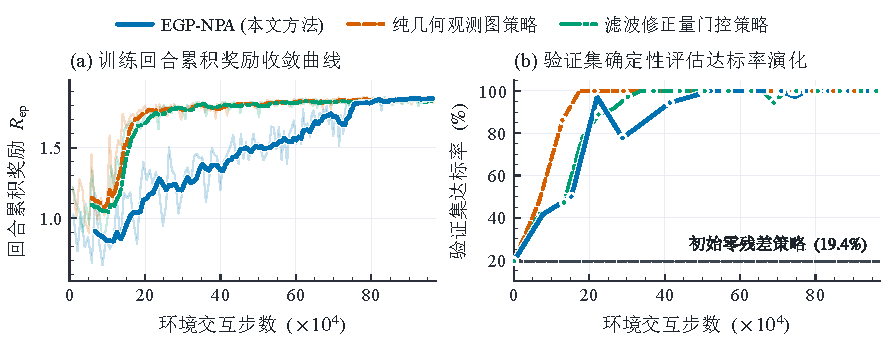
\includegraphics[width=\textwidth]{figures_zh/fig2_training_curves.pdf}
\caption{完整预算下原策略与另行训练配置的回报及验证成功率。每条曲线对应一次训练，不代表跨训练种子的均值与置信区间。}\label{fig:train-curves}
\end{figure*}

\begin{table*}[t]
\centering\footnotesize
\caption{指定冻结策略与解析参照在 $N=8$ 开发基准上的表现；时间为安全到达运行的中位数}\label{tab:e1}
\begin{tabularx}{\textwidth}{@{}Xcccccc@{}}\toprule
控制器 & $f=.60$ 到达 & 时间/s & $f=.90$ 到达 & 时间/s & 步长减半 & 审计失败段\\\midrule
EGP-NPA，$B=8$ & $32/32$ & $7.32$ & $32/32$ & $7.12$ & $0$ & $0$\\
常值切向残差 + NPA，$B=8$ & $21/32$ & $32.50$ & $18/32$ & $30.50$ & $0$ & $0$\\
比例吸引 + NPA，$B=8$ & $17/32$ & $36.35$ & $16/32$ & $31.80$ & $0$ & $0$\\
\bottomrule\end{tabularx}
\end{table*}

\begin{table*}[t]
\centering\footnotesize
\caption{指定冻结策略与解析参照的跨规模表现；括号内为安全到达时间中位数/s}\label{tab:e2}
\begin{tabularx}{\textwidth}{@{}Xccccr@{}}\toprule
控制器 & $N=12$ & $N=20$ & $N=25$ & 合计 & 步长减半\\\midrule
EGP-NPA，$B=8$ & $12/12\ (6.52)$ & $12/12\ (10.55)$ & $8/8\ (10.43)$ & $32/32$ & $0$\\
常值切向残差 + NPA & $7/12\ (14.40)$ & $4/12\ (24.53)$ & $2/8\ (38.22)$ & $13/32$ & $14198$\\
比例吸引 + NPA & $4/12\ (34.30)$ & $1/12\ (55.50)$ & $0/8\ (\text{---})$ & $5/32$ & $0$\\
\bottomrule\end{tabularx}
\end{table*}

表\ref{tab:e1}与表\ref{tab:e2}表明，该冻结策略在开发任务中取得 $96/96$ 安全到达；另一个含 $48$ 个任务的留出集合上取得 $48/48$。这里的 $100\%$ 描述指定检查点在这些任务上的观测表现。该检查点不与较少预算训练模型混合用于算法优越性排名；训练随机性由下述匹配实验单独考察。

\subsection{同预算、同种子的学习变体比较}\label{subsec:matched}
采用 $2\times2$ 析因设计，分别改变团队/局部价值网络及投影正则的开/关，每格训练两次。各配置共享 $17$ 维节点与 $20$ 维边观测、两层等变图策略、训练分布、奖励、每拍训练分配轮数 $B=2$ 和验证选模规则；相同编号的重复使用匹配的初始化与场景随机数种子。每次分配 $4.8\times10^5$ 环境步预算，按完整采样批次结束，实际训练步数范围为 $481274$--$487089$。全部八个检查点在同一 $48$ 个留出任务上以完成包络和 $B=8$ 评测，共 $384$ 次运行，未出现审计失败或步长减半。

投影正则项为 $\mathcal L_{\mathrm{proj}}=\lambda_{\mathrm{proj}}N^{-1}\sum_i\norm{\Pi_{\mathcal U_i}(\bu_i^{\mathrm{nom}})-\operatorname{sg}(\bu_i)}_2^2$，取 $\lambda_{\mathrm{proj}}\in\{0,1\}$，$\operatorname{sg}$ 表示停止梯度。权重依据训练前的梯度尺度标定。两种权重均按同一验证指标选模，所得检查点阶段仍有差异：团队价值网络无正则组约在 $21.6/40.1$ 万步选中，有正则组约在 $7.1/7.3$ 万步选中；局部价值网络对应约 $36.0/42.0$ 万步与 $14.0/12.9$ 万步。比较对象因此是包含验证选模的训练流程。

\begin{table*}[t]
\centering\footnotesize
\caption{匹配预算的内部学习变体。分号分隔两次训练重复；时间差为同种子共同安全到达任务上的“正则组减基础组”，单位 s}\label{tab:matched}
\begin{tabularx}{\textwidth}{@{}Xcccc@{}}\toprule
价值网络 & $\lambda_{\mathrm{proj}}$ & $N=8$ 安全到达 & 跨规模安全到达 & 配对中位时间差\\\midrule
团队 & 0 & $32/32\ ;\ 32/32$ & $12/16\ ;\ 14/16$ & --- \\
团队 & 1 & $32/32\ ;\ 32/32$ & $9/16\ ;\ 11/16$ & $+0.00\ ;\ +1.60$ \\
局部 & 0 & $32/32\ ;\ 32/32$ & $4/16\ ;\ 9/16$ & --- \\
局部 & 1 & $31/32\ ;\ 32/32$ & $8/16\ ;\ 14/16$ & $+4.35\ ;\ +1.60$ \\
\bottomrule\end{tabularx}
\end{table*}

表\ref{tab:matched}显示明确的交互现象：团队价值网络下，正则组两次训练均少到达 $3$ 个跨规模任务；局部价值网络下，正则组的跨规模到达数分别由 $4$ 增至 $8$、由 $9$ 增至 $14$。共同到达时间差分别为 $0.00/1.60\ \mathrm s$ 与 $4.35/1.60\ \mathrm s$。把跨规模未到达计为 $60\ \mathrm s$ 后，团队组平均完成时间由 $28.23/20.49\ \mathrm s$ 变为 $34.10/29.34\ \mathrm s$，局部组则由 $50.42/35.11\ \mathrm s$ 改善至 $39.32/22.88\ \mathrm s$。因此，投影正则降低干预量的效果与任务到达表现需要分别评价；当前两个训练重复支持配置交互的描述，尚不足以给出算法级显著性结论。

\begin{figure*}[t]
\centering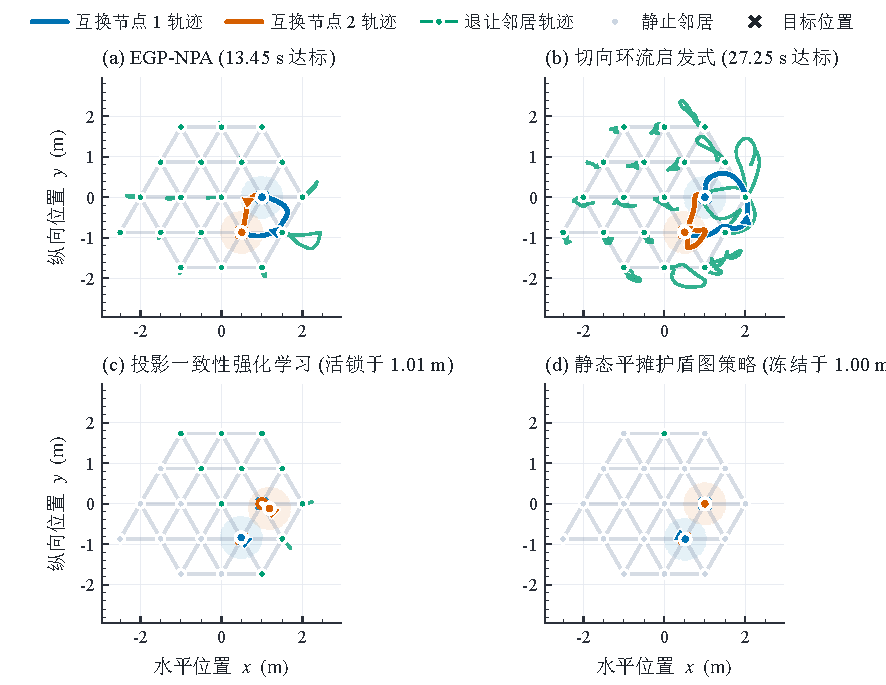
\includegraphics[width=\textwidth]{figures_zh/fig3_swap_trajectory.pdf}
\caption{同一 $N=20$ 留出互换任务上、相同预算的团队价值网络策略轨迹。(a)--(b) 第一次训练的基础组与投影正则组；(c)--(d) 第二次训练的对应配对。所有面板采用相同初始状态、目标、安全参数与坐标范围。}\label{fig:swap-traj}
\end{figure*}
\begin{figure*}[t]
\centering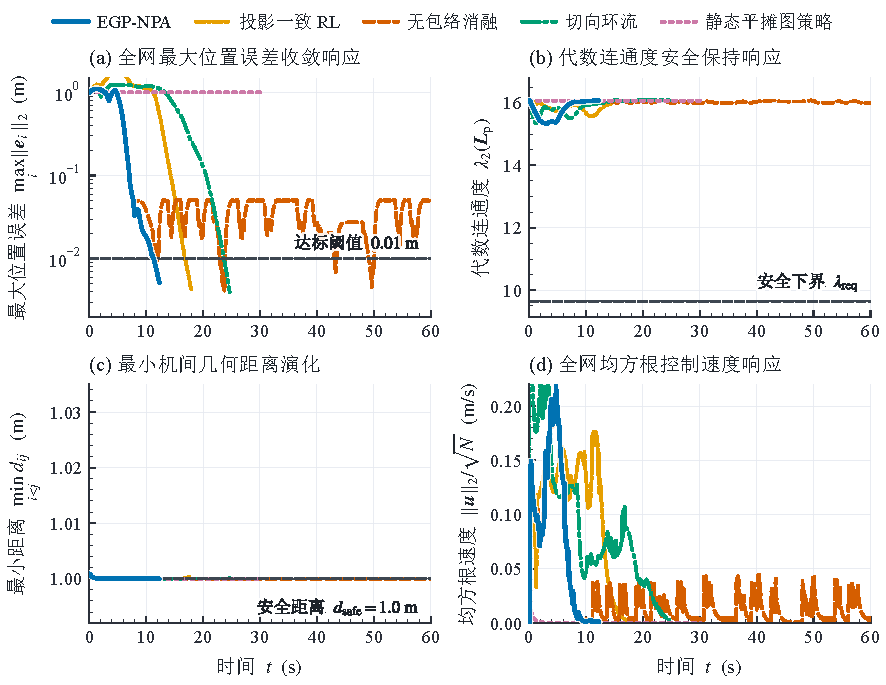
\includegraphics[width=\textwidth]{figures_zh/fig4_time_evolution.pdf}
\caption{图\ref{fig:swap-traj}同一任务及四个匹配配置的时间响应：最大目标误差、代数连通度、最小机间距离与均方根速度。曲线直接来自保存的执行轨迹，运行终止后不补画延长段。}\label{fig:time-evol}
\end{figure*}

\subsection{固定权重消融与失效类型}\label{subsec:ablation}
保持原始策略权重不变，将 NPA 分配轮数由 $B=8$ 改为 $B=0$，所得静态分配消融在 $N=8$ 与跨规模任务分别安全到达 $11/64$ 与 $1/32$。这是在动态护盾下训练、在静态护盾下执行的组件替换，不是重新训练的独立算法。表\ref{tab:static-status}给出全部终止原因；其中 $51$ 次认证或计算预算终止应与零速停滞区分。

\begin{table}[t]
\centering\footnotesize
\caption{静态分配消融的全部终止状态}\label{tab:static-status}
\begin{tabular}{@{}lrr@{}}\toprule
终止状态 & $N=8$ & 跨规模\\\midrule
安全到达 & 11 & 1\\
认证停止 & 30 & 7\\
控制调用预算耗尽 & 7 & 7\\
零速停滞 & 12 & 13\\
物理时域超时 & 4 & 4\\\bottomrule
\end{tabular}
\end{table}

在一个 $N=20$ 互换任务的早期 $[0.05,1.00]\ \mathrm s$ 内，保持相同标称输入时，动态/静态分配的待互换节点侧向执行速度分别为 $0.2003/0.0004\ \mathrm{m/s}$，外围邻居向外执行速度分别为 $0.0915/0.0013\ \mathrm{m/s}$。这一局部对照与命题\ref{prop:unfreeze}的两节点退让机制一致；复杂多接触任务的失败类型仍按表\ref{tab:static-status}报告。

\begin{table*}[t]
\centering\footnotesize
\caption{给定策略的内部干预；不同训练检查点与固定权重干预分别标明}\label{tab:decomp}
\begin{tabularx}{\textwidth}{@{}Xlc@{}}\toprule
配置 & 比较方式 & 安全到达\\\midrule
完整策略与完成包络 & 参照检查点 & $32/32$\\
去除完成包络 & 固定权重，执行期替换 & $25/32$\\
纯几何观测训练 & 另一次训练检查点 & $22/32$\\
滤波修正量门控训练 & 另一次训练检查点 & $15/32$\\\midrule
原配门控 / 单包络 / 修正量门控替换 & 固定权重，16任务子集 & 各 $16/16$\\
碰撞影子价格特征置零 & 固定权重，16任务子集 & $16/16$\\
碰撞边记录置零 & 固定权重，16任务子集 & $16/16$\\
全部代数特征置零 & 固定权重，16任务子集 & $15/16$\\\bottomrule
\end{tabularx}
\end{table*}

完成包络去除后出现的终段悬停说明该组件对给定策略有实际作用。不同训练检查点的差异同时含训练随机性；执行期特征置零则检验已训练策略的敏感性，不替代重新训练后的信息价值比较。对 $48$ 个留出任务实施推理期镜像对称化后，到达数由 $48$ 变为 $30$；该结果描述此确定性策略的反射对称化干预，与严格对称迎头构型的结构分析相对应。

\begin{figure*}[t]
\centering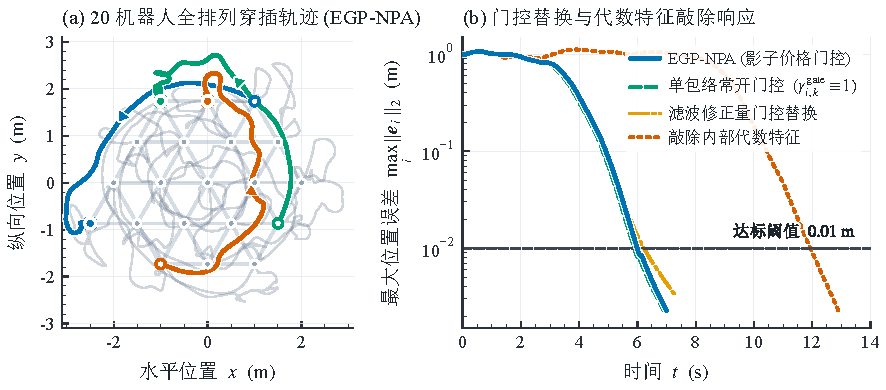
\includegraphics[width=\textwidth]{figures_zh/fig5_perm_and_gate.pdf}
\caption{给定策略的全排列任务轨迹与固定权重的门控、特征干预响应。训练配置的比较与执行期干预分别评价。}\label{fig:perm-gate}
\end{figure*}

无护盾的自建拉格朗日 PPO 作为探索性负面结果保留。该实现使用 $12/13$ 维几何输入，训练交互上限为 $264000$ 步，末次记录的平均代价约 $0.929$，尚未满足其设定的 $0.02$ 约束限额。在统一为实际保持 $1.0\ \mathrm s$、取消位置边界裁剪后重新评测，同一检查点在 $96$ 个开发任务中仍均发生碰撞。该结果说明此训练配置尚不能满足任务约束；不据此判断原始--对偶安全学习的一般能力，也不将其作为本文方法必要性的证明。

\subsection{二阶物理仿真的独立边界检验}\label{subsec:mujoco}
二阶验证采用 \texttt{MuJoCo} 刚体动力学，质量 $6.0\ \mathrm{kg}$、车体半径 $0.45\ \mathrm m$、速度环时间常数 $45\ \mathrm{ms}$、推力上限 $22.0\ \mathrm N$、物理积分周期 $5\ \mathrm{ms}$ 和控制周期 $50\ \mathrm{ms}$。在线谱估计每拍执行六轮一致性更新，NPA 执行四轮；观测延迟为 $10\ \mathrm{ms}$，通信延迟为 $5$--$15\ \mathrm{ms}$，丢包率为 $2\%$。这些实验与单积分器比较分开报告。

\begin{table*}[t]
\centering\footnotesize
\caption{两档物理参数下的到达与安全边界。到达未附加无违约条件；距离为四任务最小值，违约步数为四任务平均值}\label{tab:mujoco}
\begin{tabularx}{\textwidth}{@{}lcXcrr@{}}\toprule
档位 & 规模 & 配置 & 到达 & 最小距离/m & 违约步数\\\midrule
A & 8 & 比例吸引 + 物理接口 & $0/4$ & .9817 & 610.2\\
A & 8 & 学习策略 + 静态分配 & $1/4$ & .9798 & 442.2\\
A & 8 & 学习策略 + 无补偿滤波 & $0/4$ & .9792 & 4231.0\\
A & 8 & 学习策略 + 在线谱估计 + 物理接口 & $3/4$ & .8990 & 1683.5\\
A & 12 & 比例吸引 + 物理接口 & $0/4$ & .9952 & 1679.2\\
A & 12 & 学习策略 + 静态分配 & $0/4$ & .9976 & 850.8\\
A & 12 & 学习策略 + 无补偿滤波 & $0/4$ & .9937 & 4190.2\\
A & 12 & 学习策略 + 在线谱估计 + 物理接口 & $1/4$ & .8988 & 2777.0\\\midrule
B & 8 & 比例吸引 + 物理接口 & $0/4$ & 1.0240 & 0\\
B & 8 & 学习策略 + 静态分配 & $0/4$ & 1.0260 & 0\\
B & 8 & 学习策略 + 无补偿滤波 & $0/4$ & .8987 & 4722.0\\
B & 8 & 学习策略 + 在线谱估计 + 物理接口 & $0/4$ & .9910 & 1133.2\\
B & 12 & 比例吸引 + 物理接口 & $0/4$ & 1.0256 & 0\\
B & 12 & 学习策略 + 静态分配 & $0/4$ & 1.0255 & 0\\
B & 12 & 学习策略 + 无补偿滤波 & $0/4$ & .9809 & 4783.2\\
B & 12 & 学习策略 + 在线谱估计 + 物理接口 & $0/4$ & 1.0096 & 0\\\bottomrule
\end{tabularx}
\end{table*}

档位 A 的初始格距为 $1.018\ \mathrm m$；档位 B 取 $1.045\ \mathrm m$、距离收紧 $0.028\ \mathrm m$ 和速度增量限幅 $0.22\ \mathrm{m/s}$。表\ref{tab:mujoco}完整保留了全栈方法的负面结果：A 档虽有到达，但存在安全距离越界；B 档八个任务均未到达，其中七个没有碰撞距离违约，另一个 $N=8$ 任务最小距离为 $0.9910\ \mathrm m$。全部 $64$ 次物理运行的连通违约记录为零。谱估计跟踪误差小并不意味着避碰约束同时满足，单积分器安全结论也不直接适用于含执行器滞后和后置限幅的系统。

\begin{figure*}[t]
\centering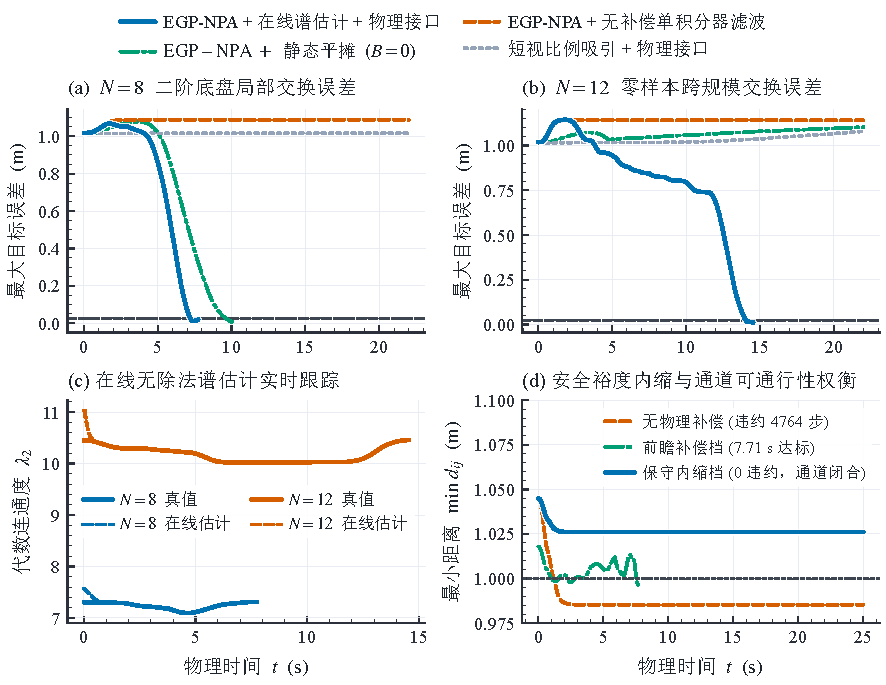
\includegraphics[width=\textwidth]{figures_zh/fig6_mujoco_verification.pdf}
\caption{二阶物理闭环的目标误差、在线谱估计与距离响应。不同补偿档位均保留原始越界与未到达结果。}\label{fig:mujoco}
\end{figure*}

\begin{theorem}[收紧距离下的初始可行性与指定交会截面]\label{thm:passability-tradeoff}
记 $D=\ds+\Delta d_{\mathrm{phys}}$。最小初始格距为 $S$ 时，所有距离约束严格可行当且仅当 $D<S$。进一步，仅考虑四节点位于同心垂直对角线两端、移动节点对角线长度固定为 $D$ 的对称交会截面；若另外一条对角线为 $b$，全部相邻距离不小于 $D$ 当且仅当 $b\ge\sqrt3D$。
\end{theorem}
\begin{proof}
第一项由最小初始距离定义直接得到。指定截面的每条相邻边长度为 $\sqrt{D^2+b^2}/2$，故其不小于 $D$ 等价于 $b^2\ge3D^2$。另外两条对角线分别为 $D$ 与 $b\ge\sqrt3D$，也满足距离要求。
\end{proof}
该定理给出指定截面的几何条件。一般重排任务还允许非对称绕行与外围整体移动，完整构型空间是否道路连通需另行分析，不能仅由该截面的孔径条件推断。
